\section{From range to engineering}
\label{sec:engineering}

\paragraph{Propulsion sets speed, lifetime sets range.} A rocket that must
accelerate \emph{and} brake on one tank with mass ratio $R$ and exhaust speed
$v_e$ cruises at $v=c\tanh(v_e\ln R/2c)$ (relativistic rocket equation, half
the rapidity on each burn). Its hop range is $r=v\,\tau_{\max}$, where
$\tau_{\max}$ is how long the ship, or its crew, survives in transit. The
per-hop survival time needed to percolate is therefore $\tau^\ast=r_{50}/v$
(Figure~\ref{fig:propulsion}). At $R=10$, chemical rockets need
\TauChemStatic~yr per hop and high-$I_{\rm sp}$ electric propulsion
\TauElecStatic~yr. A Daedalus-class fusion ship ($v_e=10^4$~km/s, cruising at
\VFusion~km/s, \VFusionPctC\% of $c$) needs \TauFusionStatic~yr, and an
idealised antimatter ship \TauAntiStatic~yr. If colonies can wait up to
\MovingTkyr~kyr for good alignments, every requirement roughly halves (fusion:
\TauFusionMoving~yr). This turns a technology into a reachability statement:
\emph{fusion propulsion and century-scale reliability are enough to percolate
through the solar neighbourhood}.

\begin{figure}[t]
\centering
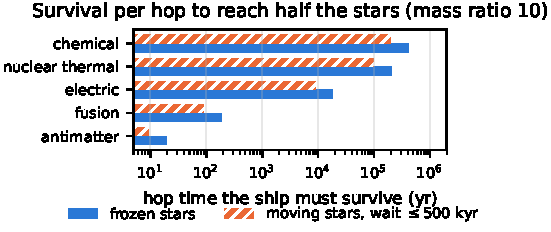
\includegraphics[width=\linewidth]{figures/propulsion.pdf}
\caption{Hop time a ship must survive to reach half the stars within
\EvalRadius~pc, by propulsion technology (mass ratio 10, accelerate and brake
on one tank). Hatched bars: colonies may wait up to \MovingTkyr~kyr for stars
to drift into range.}
\label{fig:propulsion}
\end{figure}

\paragraph{Pilots: greedy fails near threshold, A* is cheap.} On the static
range graph, a greedy geographic pilot (always hop to the in-range neighbour
closest to the target) reaches only \GreedyTwoFive\% of random targets at
$r=2.5$~pc and \GreedyThree\% at 3~pc. It gets stuck in local minima, the
``voids'' known from wireless routing \cite{bose2001routing}. It succeeds
\GreedyFour\% of the time at 4~pc. Near threshold, optimal routes are winding
(median stretch \OptStretchTwoFive\ at 2.5~pc), so a heuristic that never
moves away from the target is wrong by design. A* with the straight-line
heuristic finds the same optimal routes as Dijkstra while expanding a median
of \AstarRatioTwoFive\% of Dijkstra's nodes at 2.5~pc and \AstarRatioFour\% at
4~pc.

\paragraph{Refuelling only where planets are known.} Suppose a ship may stop
anywhere, with hops of at most \FuelHop~pc for crew or hardware reasons, but
can refuel only at the \NHostsFuel\ known exoplanet hosts within
\FuelRadius~pc. The tank range then needed to reach each star is again a
bottleneck, now on a station graph whose edge weights are in-graph shortest
distances. We compute it exactly by multi-source Dijkstra and an MST over
stations. Reaching half the stars needs a \TankFifty~pc tank (90\%:
\TankNinety~pc), \TankRatio$\times$ the \RefuelAnyFifty~pc that suffices when
any star can refuel (Figure~\ref{fig:routing}, left). Planet surveys therefore
shorten the required tank directly: every newly confirmed host is a potential
refuelling station.

\begin{figure*}[t]
\centering
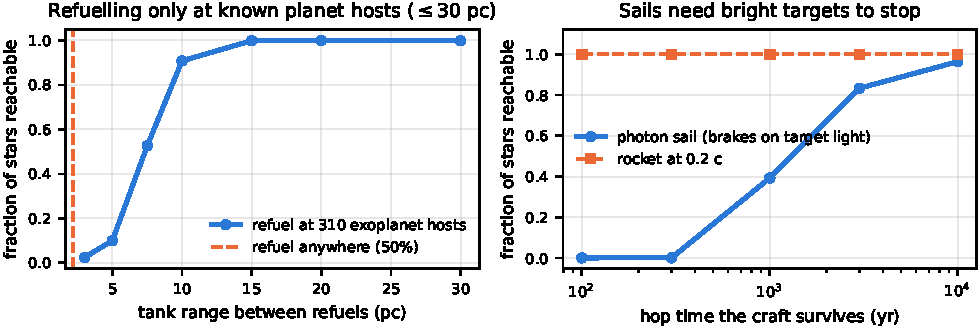
\includegraphics[width=\textwidth]{figures/routing.pdf}
\caption{\textbf{Left:} reach within \EvalRadius~pc against tank range when
refuelling is possible only at known exoplanet hosts (hops $\le$\FuelHop~pc).
The dashed line is $r_{50}$ when any star can refuel. \textbf{Right:} photon
sails launched at \SailVLaunch~$c$ but braking only on the target star's light,
against a rocket flying at the same speed. Reach is plotted against the hop
time the craft survives.}
\label{fig:routing}
\end{figure*}

\paragraph{Sails need bright targets.} A laser-launched sail can leave at
\SailVLaunch~$c$, but to stop it must shed its speed on the target's light.
Scaling the photogravitational braking limit of \cite{heller2017optimized}
(13,800~km/s at $\alpha$~Cen~A) as $L^{0.4}$, the median star within
\EvalRadius~pc can stop a sail arriving at only \SailBrakeMedian~km/s. Only
\SailFracFast\% can stop one faster than 0.01~$c$, because most nearby stars
are M dwarfs. Sail routes therefore hop between bright stars or crawl into dim
ones. With a 1,000-yr hop budget a sail network reaches \SailReachThousand\% of
stars, against 100\% for a rocket at the same cruise speed. At 3,000~yr it
reaches \SailReachThreeThousand\%, and half the stars take \SailTFifty~yr
rather than \RocketTFifty~yr (Figure~\ref{fig:routing}, right).

\paragraph{Exploring everything nearby.} Finally we reproduce the classic
probe-exploration model of Bj{\o}rk \cite{bjork2007exploring}. A fleet splits
the sky into sectors, and each probe visits every star in its sector, here
the \ExNStars\ stars within \ExRadius~pc. Replacing the nearest-neighbour rule
with 2-opt local search shortens total flight by \TwoOptMin--\TwoOptMax\%
across fleet sizes of 1--16, consistent with the $\sim$10\% of
\cite{cotta2009computational} on synthetic stars
(Figure~\ref{fig:exploration}). Against the MST lower bound, nearest-neighbour
tours are \NNGapOne\% too long and 2-opt tours \OptGapOne\%. At 0.1~$c$ a
single probe needs \MakespanOneKyr~kyr to visit them all. A fleet of
\FleetBig\ needs \MakespanEightKyr~kyr. Fleet parallelism, not tour quality,
dominates exploration time.

\begin{figure}[t]
\centering
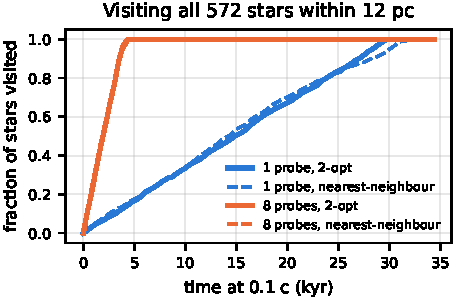
\includegraphics[width=\linewidth]{figures/exploration.pdf}
\caption{Fraction of stars within \ExRadius~pc visited over time by 1 and
\FleetBig\ probes at 0.1~$c$: 2-opt tours (solid) against the nearest-neighbour
rule (dashed).}
\label{fig:exploration}
\end{figure}
